\documentclass{article}

\usepackage{fancyhdr}
\usepackage{extramarks}
\usepackage{amsmath}
\usepackage{amsthm}
\usepackage{amsfonts}
\usepackage{tikz}
\usepackage{graphicx} %插入图片的宏包
\usepackage{float} %设置图片浮动位置的宏包
\usepackage{pythonhighlight}
% \usepackage{subfigure} %插入多图时用子图显示的宏包
% \usepackage[plain]{algorithm}
% \usepackage{algpseudocode}

% \usetikzlibrary{automata,positioning}

%
% Basic Document Settings
%

\topmargin=-0.45in
\evensidemargin=0in
\oddsidemargin=0in
\textwidth=6.5in
\textheight=9.0in
\headsep=0.25in

\linespread{1.1}

\pagestyle{fancy}
\lhead{\hmwkAuthorName}
\chead{\hmwkClass\ : \hmwkTitle}
\rhead{\firstxmark}
\lfoot{\lastxmark}
\cfoot{\thepage}

\renewcommand\headrulewidth{0.4pt}
\renewcommand\footrulewidth{0.4pt}

\setlength\parindent{0pt}


%代码格式设置



%
% Create Problem Sections
%

\newcommand{\enterProblemHeader}[1]{
    \nobreak\extramarks{}{Problem \arabic{#1} continued on next page\ldots}\nobreak{}
    \nobreak\extramarks{Problem \arabic{#1} (continued)}{Problem \arabic{#1} continued on next page\ldots}\nobreak{}
}

\newcommand{\exitProblemHeader}[1]{
    \nobreak\extramarks{Problem \arabic{#1} (continued)}{Problem \arabic{#1} continued on next page\ldots}\nobreak{}
    \stepcounter{#1}
    \nobreak\extramarks{Problem \arabic{#1}}{}\nobreak{}
}

\setcounter{secnumdepth}{0}
\newcounter{partCounter}
\newcounter{homeworkProblemCounter}
\setcounter{homeworkProblemCounter}{1}
\nobreak\extramarks{Problem \arabic{homeworkProblemCounter}}{}\nobreak{}

%
% Homework Problem Environment
%
% This environment takes an optional argument. When given, it will adjust the
% problem counter. This is useful for when the problems given for your
% assignment aren't sequential. See the last 3 problems of this template for an
% example.
%
\newenvironment{homeworkProblem}[1][-1]{
    \ifnum#1>0
        \setcounter{homeworkProblemCounter}{#1}
    \fi
    \section{Problem \arabic{homeworkProblemCounter}}
    \setcounter{partCounter}{1}
    \enterProblemHeader{homeworkProblemCounter}
}{
    \exitProblemHeader{homeworkProblemCounter}
}

%
% Homework Details
%   - Title
%   - Due date
%   - Class
%   - Section/Time
%   - Instructor
%   - Author
%

\newcommand{\hmwkTitle}{Quiz\ \#9}
\newcommand{\hmwkDueDate}{Jan 16th, 2019}
\newcommand{\hmwkClass}{Complex Networks}
\newcommand{\hmwkClassTime}{Section A}
% \newcommand{\hmwkClassInstructor}{Professor Isaac Newton}
\newcommand{\hmwkAuthorName}{\textbf{RUOPENG XU} }
\newcommand{\hmwkAuthorNum}{\textbf{18M38179} }

%
% Title Page
%

\title{
    \vspace{2in}
    \textmd{\textbf{\hmwkClass:\ \hmwkTitle}}\\
    \normalsize\vspace{0.1in}\small{Due\ on\ \hmwkDueDate\ }\\
    % \vspace{0.1in}\large{\textit{\hmwkClassInstructor\ \hmwkClassTime}}
    \vspace{3in}
}

\author{\hmwkAuthorName\\ \hmwkAuthorNum}
\date{}

\renewcommand{\part}[1]{\textbf{\large Part \Alph{partCounter}}\stepcounter{partCounter}\\}

%
% Various Helper Commands
%

% Useful for algorithms
\newcommand{\alg}[1]{\textsc{\bfseries \footnotesize #1}}

% For derivatives
\newcommand{\deriv}[1]{\frac{\mathrm{d}}{\mathrm{d}x} (#1)}

% For partial derivatives
\newcommand{\pderiv}[2]{\frac{\partial}{\partial #1} (#2)}

% Integral dx
\newcommand{\dx}{\mathrm{d}x}

% Alias for the Solution section header
\newcommand{\solution}{\textbf{\large Solution}}

% Probability commands: Expectation, Variance, Covariance, Bias
\newcommand{\E}{\mathrm{E}}
\newcommand{\Var}{\mathrm{Var}}
\newcommand{\Cov}{\mathrm{Cov}}
\newcommand{\Bias}{\mathrm{Bias}}

\begin{document}

\maketitle

\pagebreak

\begin{homeworkProblem}
    % questions
Make a program of Dijkstra’s algorithm without
built-in functions (dijkstra\_path \& dijkstra\_path\_length).

% 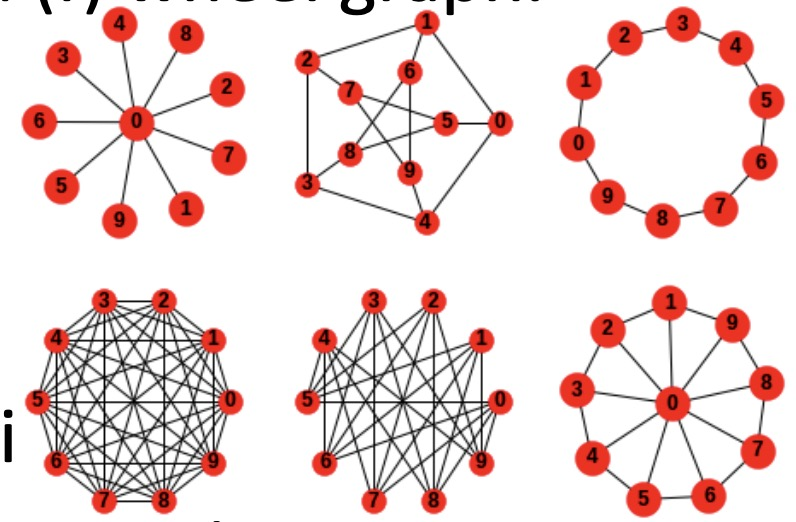
\includegraphics[scale=0.3]{quiz6_1.jpg}

\subsection*{Answer 1}
% 使用BFS来进行最短路径的问题(从起点到终点),在加权的图上面,找到cost最少的路线
% 初始的点上赋值是0,其他的点都是无穷
% 一个visted set和一个unvisited set. current的点计算他的所有unvisited的(到这个点的距离)+ (从这个点到邻居的距离)。如果比现在的小就更新这个点的距离
% 找到现在身上带着数字的最小的然后把新的点更新到visited


\begin{python}
import networkx as nx
import matplotlib.pyplot as plt
import numpy as np
import sys
import functools
import operator

G = nx.Graph()
G.add_nodes_from(range(0, 5))
G.add_weighted_edges_from([(0, 1, 7), (0, 2, 9), (0, 5, 14), (1, 2, 10), (1, 3, 15), (2, 3, 11), (2, 5, 2), (3, 4, 6), (4, 5, 9)])

plt.figure(figsize=(5, 5))
pos = nx.spring_layout(G)
nx.draw_networkx_edges(G, pos)
nx.draw_networkx_nodes(G, pos)
nx.draw_networkx_edge_labels(G, pos, font_size=16, edge_labels={(u, v): d["weight"] for u, v, d in G.edges(data=True)})
nx.draw_networkx_labels(G, pos)
plt.axis('off')
plt.show()

# find the smallest one
dist_estimate = [sys.maxsize] * nx.number_of_nodes(G) 
# real distance
dist_certainty = [0] * nx.number_of_nodes(G)
dist_estimate[1] = 0


print(dist_estimate)
print(dist_certainty)

#
# please fill in this part (Dijkstra's algorithm)
# calculte the distance from 1 -> 4

n = 0
distance = 0
count = 1
temp_nodes = 0

for visited in dist_certainty:
  if (visited <= 1 ):
# find the smallest estimate in G
    for nodes in G:
      if (dist_certainty[nodes] == 0):
          temp_min = dist_estimate[nodes]
          break
    for nodes in G:
      if (dist_certainty[nodes] == 0):
        if (dist_estimate[nodes] <= temp_min and dist_estimate[nodes] < 10000):
          temp_min = dist_estimate[nodes]
          temp_node = nodes
    current_distance = temp_min
    current_node = temp_node
      
    print("In step",count,":")
    print("current_distance = ", current_distance)
    print("current_node = ", current_node)

  #     mark this distance as certain
    dist_certainty[current_node] = 1
  #     calculate the distance and compare     
    for neighbor in G.neighbors(current_node):
      if (dist_certainty[neighbor] != 1):
        weight = list(dict.values(G.get_edge_data(current_node,neighbor)))
        current_weight = int(weight[0])
        distance = current_distance + current_weight
        if(distance < dist_estimate[neighbor]):
          dist_estimate[neighbor] = distance

    print("dist_estimate",dist_estimate)
    print("dist_certainty",dist_certainty)
    count = count + 1





#######
# print(dist_estimate)
# print(dist_certainty)
print("From built-in function:")
print(nx.dijkstra_path(G,1,4))
print(nx.dijkstra_path_length(G,1,4))
\end{python}

The result is:
\begin{python}
[9223372036854775807, 0, 9223372036854775807, 9223372036854775807, 9223372036854775807, 9223372036854775807]
[0, 0, 0, 0, 0, 0]
In step 1 :
current_distance =  0
current_node =  1
dist_estimate [7, 0, 10, 15, 9223372036854775807, 9223372036854775807]
dist_certainty [0, 1, 0, 0, 0, 0]
In step 2 :
current_distance =  7
current_node =  0
dist_estimate [7, 0, 10, 15, 9223372036854775807, 21]
dist_certainty [1, 1, 0, 0, 0, 0]
In step 3 :
current_distance =  10
current_node =  2
dist_estimate [7, 0, 10, 15, 9223372036854775807, 12]
dist_certainty [1, 1, 1, 0, 0, 0]
In step 4 :
current_distance =  12
current_node =  5
dist_estimate [7, 0, 10, 15, 21, 12]
dist_certainty [1, 1, 1, 0, 0, 1]
In step 5 :
current_distance =  15
current_node =  3
dist_estimate [7, 0, 10, 15, 21, 12]
dist_certainty [1, 1, 1, 1, 0, 1]
In step 6 :
current_distance =  21
current_node =  4
dist_estimate [7, 0, 10, 15, 21, 12]
dist_certainty [1, 1, 1, 1, 1, 1]
From built-in function:
[1, 2, 5, 4]
21
\end{python}







\end{homeworkProblem}
\pagebreak


\begin{homeworkProblem}
Show all the statuses of current estimates and their certainties while Dijkstra’s algorithm is performed from vertex 0.

\subsection*{Answer 2}
According to the algorithm above, when the Dijkstra is from vertex 0, change dist\_estimate[0] to 0.
\\
The result is:
\begin{python}
In step 1 :
current_distance =  0
current_node =  0
dist_estimate [0, 7, 9, 9223372036854775807, 9223372036854775807, 14]
dist_certainty [1, 0, 0, 0, 0, 0]
In step 2 :
current_distance =  7
current_node =  1
dist_estimate [0, 7, 9, 22, 9223372036854775807, 14]
dist_certainty [1, 1, 0, 0, 0, 0]
In step 3 :
current_distance =  9
current_node =  2
dist_estimate [0, 7, 9, 20, 9223372036854775807, 11]
dist_certainty [1, 1, 1, 0, 0, 0]
In step 4 :
current_distance =  11
current_node =  5
dist_estimate [0, 7, 9, 20, 20, 11]
dist_certainty [1, 1, 1, 0, 0, 1]
In step 5 :
current_distance =  20
current_node =  4
dist_estimate [0, 7, 9, 20, 20, 11]
dist_certainty [1, 1, 1, 0, 1, 1]
In step 6 :
current_distance =  20
current_node =  3
dist_estimate [0, 7, 9, 20, 20, 11]
dist_certainty [1, 1, 1, 1, 1, 1]
From built-in function:
[0, 2, 5, 4]
20
\end{python}
\end{homeworkProblem}
\pagebreak


\begin{homeworkProblem}
Start from vertex 1 and show all the statuses \& their certainties.

\subsection*{Answer 3}
The result is same as the result in Problem 1:
\begin{python}
In step 1 :
current_distance =  0
current_node =  1
dist_estimate [7, 0, 10, 15, 9223372036854775807, 9223372036854775807]
dist_certainty [0, 1, 0, 0, 0, 0]
In step 2 :
current_distance =  7
current_node =  0
dist_estimate [7, 0, 10, 15, 9223372036854775807, 21]
dist_certainty [1, 1, 0, 0, 0, 0]
In step 3 :
current_distance =  10
current_node =  2
dist_estimate [7, 0, 10, 15, 9223372036854775807, 12]
dist_certainty [1, 1, 1, 0, 0, 0]
In step 4 :
current_distance =  12
current_node =  5
dist_estimate [7, 0, 10, 15, 21, 12]
dist_certainty [1, 1, 1, 0, 0, 1]
In step 5 :
current_distance =  15
current_node =  3
dist_estimate [7, 0, 10, 15, 21, 12]
dist_certainty [1, 1, 1, 1, 0, 1]
In step 6 :
current_distance =  21
current_node =  4
dist_estimate [7, 0, 10, 15, 21, 12]
dist_certainty [1, 1, 1, 1, 1, 1]
From built-in function:
[1, 2, 5, 4]
21
\end{python}
\end{homeworkProblem}
\pagebreak


\begin{homeworkProblem}
Explain the reasons why Dijkstra’s algorithm does not work for negative weight edges.

\subsection*{Answer 4}
Because when we think a vertex is visited and change its value in \textit{dist\_certainty} to 1, it will not be visited anymore. If a vertex is in visited, we will think we have already found the shortest path to this vertex. However, this doesn't work in ngetive path. For example, if a graph with negative edge is like this:

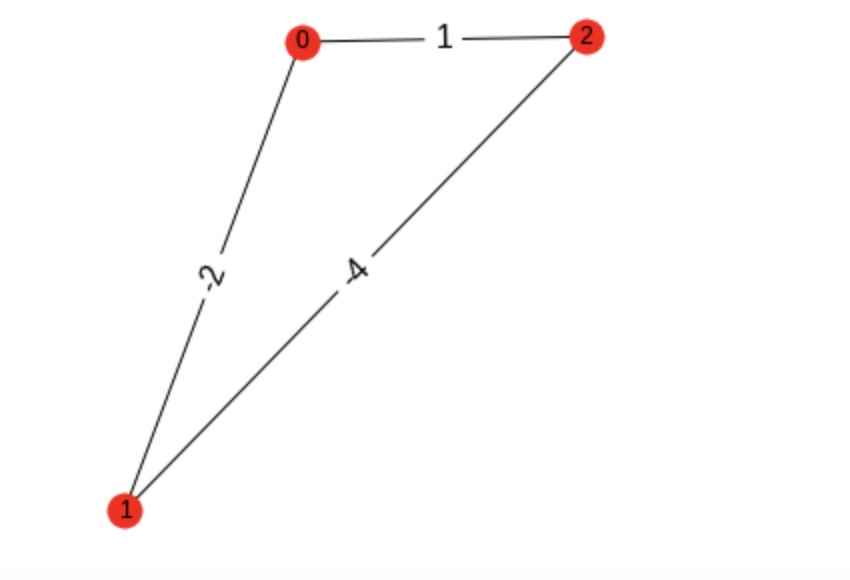
\includegraphics[scale=0.3]{quiz9_1.jpg}

When we start from vertex 0, we think the shortest path to 1 is -2, but it is actually -3(from veertex 2 to vertex 1).




\end{homeworkProblem}
\pagebreak


\end{document}
%
% Non sequential homework problems
%

% Jump to problem 18
